% Scientific Reports Article: the Introduction gives the background and
% rationale, states the contribution explicitly, and closes with the
% summary of the main results. Derived from 02_introduction_CM.tex with the
% contribution paragraph added and the framing narrowed from "a framework
% that establishes regimes" to "an instrument that returns adjudicated
% readings"; the LUAD clinical background and the mutation-prediction
% literature walk-through live in Methods and Supplementary Note 2.

\section*{Introduction}

Medical machine learning asks one modality to report on a
target it does not directly measure: histology onto
genotype,\cite{coudray2018classification,kather2020pancancer} MRI onto
molecular markers,\cite{chang2018radiogenomics} the electrocardiogram onto
physiological state.\cite{attia2019ecg} Performance on these tasks is
reported almost universally as one cohort-average \auroc{} per target.
That number conflates failures that demand opposite responses. A
target may resist prediction because the information lies \emph{outside}
the source vocabulary, because it is \emph{unestimable} at the available
positive-set size, or because it is confined to a \emph{subpopulation}
and diluted in a cohort average. The first calls for
a new source channel, the second for more data of the same kind, the third
for a change in the unit of deployment. A cohort mean renders the three
indistinguishable, and the cost is on the record: a decade of near-chance
results for MGMT-promoter methylation from preoperative MRI has
accumulated as a community-wide defeat rather than a finding, for want
of a framework in which \emph{not reachable from this modality} is
reportable.\cite{kim2022mgmtvalidation,robinet2023mgmt,saeed2023mgmt}

We propose reporting per-target \emph{translatability} instead, grounded
in an exhaustive information partition rather than a metaphor. The
construction needs two ingredients many clinical prediction tasks
already have: an \emph{expert-defined controlled vocabulary} on the source
modality, and a \emph{learned encoder} of the same modality whose
representation is unconstrained by that vocabulary
(\cref{fig:framework}). These are two sources of evidence about one
target, and partial information decomposition
(\pid{})\cite{williams2010pid,bertschinger2014unique} states the only four
ways their information can be distributed: redundantly available
from either, uniquely from one, or only from their
joint state. Which atom dominates defines three regimes. Under
\emph{encoder saturation} the vocabulary is redundant and no aggregator
converts it into a gain. Under \emph{complementarity} the vocabulary
carries what the encoder does not, either additively or---in the form an
additive head cannot express---synergistically. Under
\emph{out-of-ontology} there is no vocabulary-side atom at all, and only a
new source channel will move the target.

Two commitments make this more than a relabelling. First, we do not
estimate the atoms numerically. Direct estimation is intractable on a
$512$-dimensional source at these cohort sizes, and where attempted
across cancer cohorts it agreed with downstream performance in
one modality pair of seven.\cite{zhang2025evaluatingpid} We read each
regime from the \emph{sign} of contrasts between trained single- and
dual-channel models, and from the sign of a learned Choquet interaction
index; a sign that survives a hierarchical bootstrap over seeds and
patients is a weaker claim than a point estimate and a more reliable
one, and where none survives the instrument reports that in place of a
regime---as it does here for every lung adenocarcinoma target. Second,
the Conclusive/Inconclusive verdict is declared at the level at which it
was established. It thresholds a cohort mean, so it licenses no statement
about any named case, and is not a synonym for untranslatability.

The contribution is therefore an evaluation instrument and its
measured behaviour, not a better predictor, and we state its three
parts so that each can be weighed on its own evidence.
\emph{(1)}~A four-condition retraining protocol---encoder alone,
vocabulary alone, additive fusion, non-additive fusion---together with a
noise-aware directional rule that assigns a regime only when the deciding
contrast survives a hierarchical bootstrap and requires an explicit
equivalence test, rather than a non-significant difference, before any
``no gain'' reading is issued. Every contrast on every target is
reported with its interval (\cref{tab:luad_contrasts}), so a reader can
see which signs survive resampling and which do not.
\emph{(2)}~A falsifiable model-side signature of synergy: the non-additive
aggregator must gain on exactly the targets whose named pattern pair
co-activates, and the one target where this could be tested returned a
warranted null. \emph{(3)}~Portability of the procedure, not of any
model: with only the vocabulary and the encoder exchanged, the identical
protocol and threshold run on glioma MRI, on the electrocardiogram and
across lung adenocarcinoma cohorts, and the released code and live
deployment let any group run it on a new source--target pair. What the
instrument does \emph{not} establish is also stated: no per-target regime
assignment is reproduced across cohorts here, and the per-slide
explanation tooling released with the code is not evaluated.

Two features of the evidence are structural and are stated at the
outset because they shape every claim. First, the cohorts are the public
ones---$444$ genotyped lung adenocarcinoma patients with $30$ to $220$
positives per gene, $106$ genotyped patients in the external cohort,
$577$ glioma cases---and at these sizes no aggregator gain of the
magnitude this literature reports ($0.008$--$0.046$ \auroc{}) is
resolvable (\cref{tab:design_power}). Scarcity of this kind is the
normal condition of public histology-to-genotype work, not a defect of
one study, and the instrument is built for it: where a cohort cannot
adjudicate, its output is the sample size that could, in place of an
assignment the data do not license. Where instead the limit is the
modality rather than the cohort---every condition, the encoder alone
included, at chance---it says so without asking for more patients,
because more data narrows the interval around a contrast but does not
raise the level of a target. Second, the three regimes are a
partition of the ways two sources can share information, not a
catalogue of observed cases. Regime~(i) is adjudicated by the
equivalence rule in the electrocardiogram, the one cohort here large
enough to certify it; the modality-ceiling form of regime~(iii) is read
in glioma MGMT from every condition sitting at chance, with the verdict
resolved at full power; regime~(ii), complementarity, is occupied by
no target in any cohort here. That cell is a prediction with a stated
observation that would fill it (Methods), and an instrument that
declines to fill it on $444$ patients is behaving as specified.

We instantiate the instrument in lung adenocarcinoma, where the six ANORAK
growth patterns\cite{anorak2024} supply the vocabulary and a
foundation-model encoder\cite{wang2022ctranspath} the
unconstrained channel. Across \emph{modalities}, the same decomposition
runs unchanged on glioma MRI with the VASARI
terminology\cite{gutman2013vasari} and on the electrocardiogram with
PTB-XL's graded SCP-ECG statements,\cite{wagner2020ptbxl} including a
full-power encoder-ceiling test on MGMT. Across \emph{cohorts}, the
frozen pipeline goes off-the-shelf to CPTAC-LUAD. The first axis shows
the procedure travels; the second, that what travels is the diagnostic
rather than a frozen predictor.

In brief, on $458$ tumour slides from $444$ TCGA-LUAD patients the
instrument resolves exactly one contrast---the vocabulary channel alone
is worse than the encoder alone on \textit{TP53} and \textit{EGFR}---and
declines to assign any regime, because the design resolves only
$0.04$--$0.11$ \auroc{} per target and no deciding contrast clears that;
the per-gene reads are reported as directional, with the cohort size
that confirmation would require.
Controls show that the pipeline is calibrated (permutation null at
chance, tumour-versus-normal $0.98$) and that its ceiling is low
(\textit{TP53} $0.67$). The decomposition nonetheless separates kinds of
failure that one cohort-average number conflates: \textit{KEAP1} is at
chance on both channels, \textit{RBM10} is unestimable at $30$
positives, and the conditional test of a \textit{KRAS} synergy returns a
warranted null. In glioma MRI the same instrument declines
\textit{MGMT} at full power on $577$ cases; in the
electrocardiogram it carries two leakage-free targets intact; and under
cohort transfer it turns Inconclusive rather than issuing a confident
wrong call. We conclude that cross-domain medical prediction should be
reported with a per-target, level-explicit translatability verdict
rather than a cohort mean.

\begin{figure}[htbp]
  \centering
  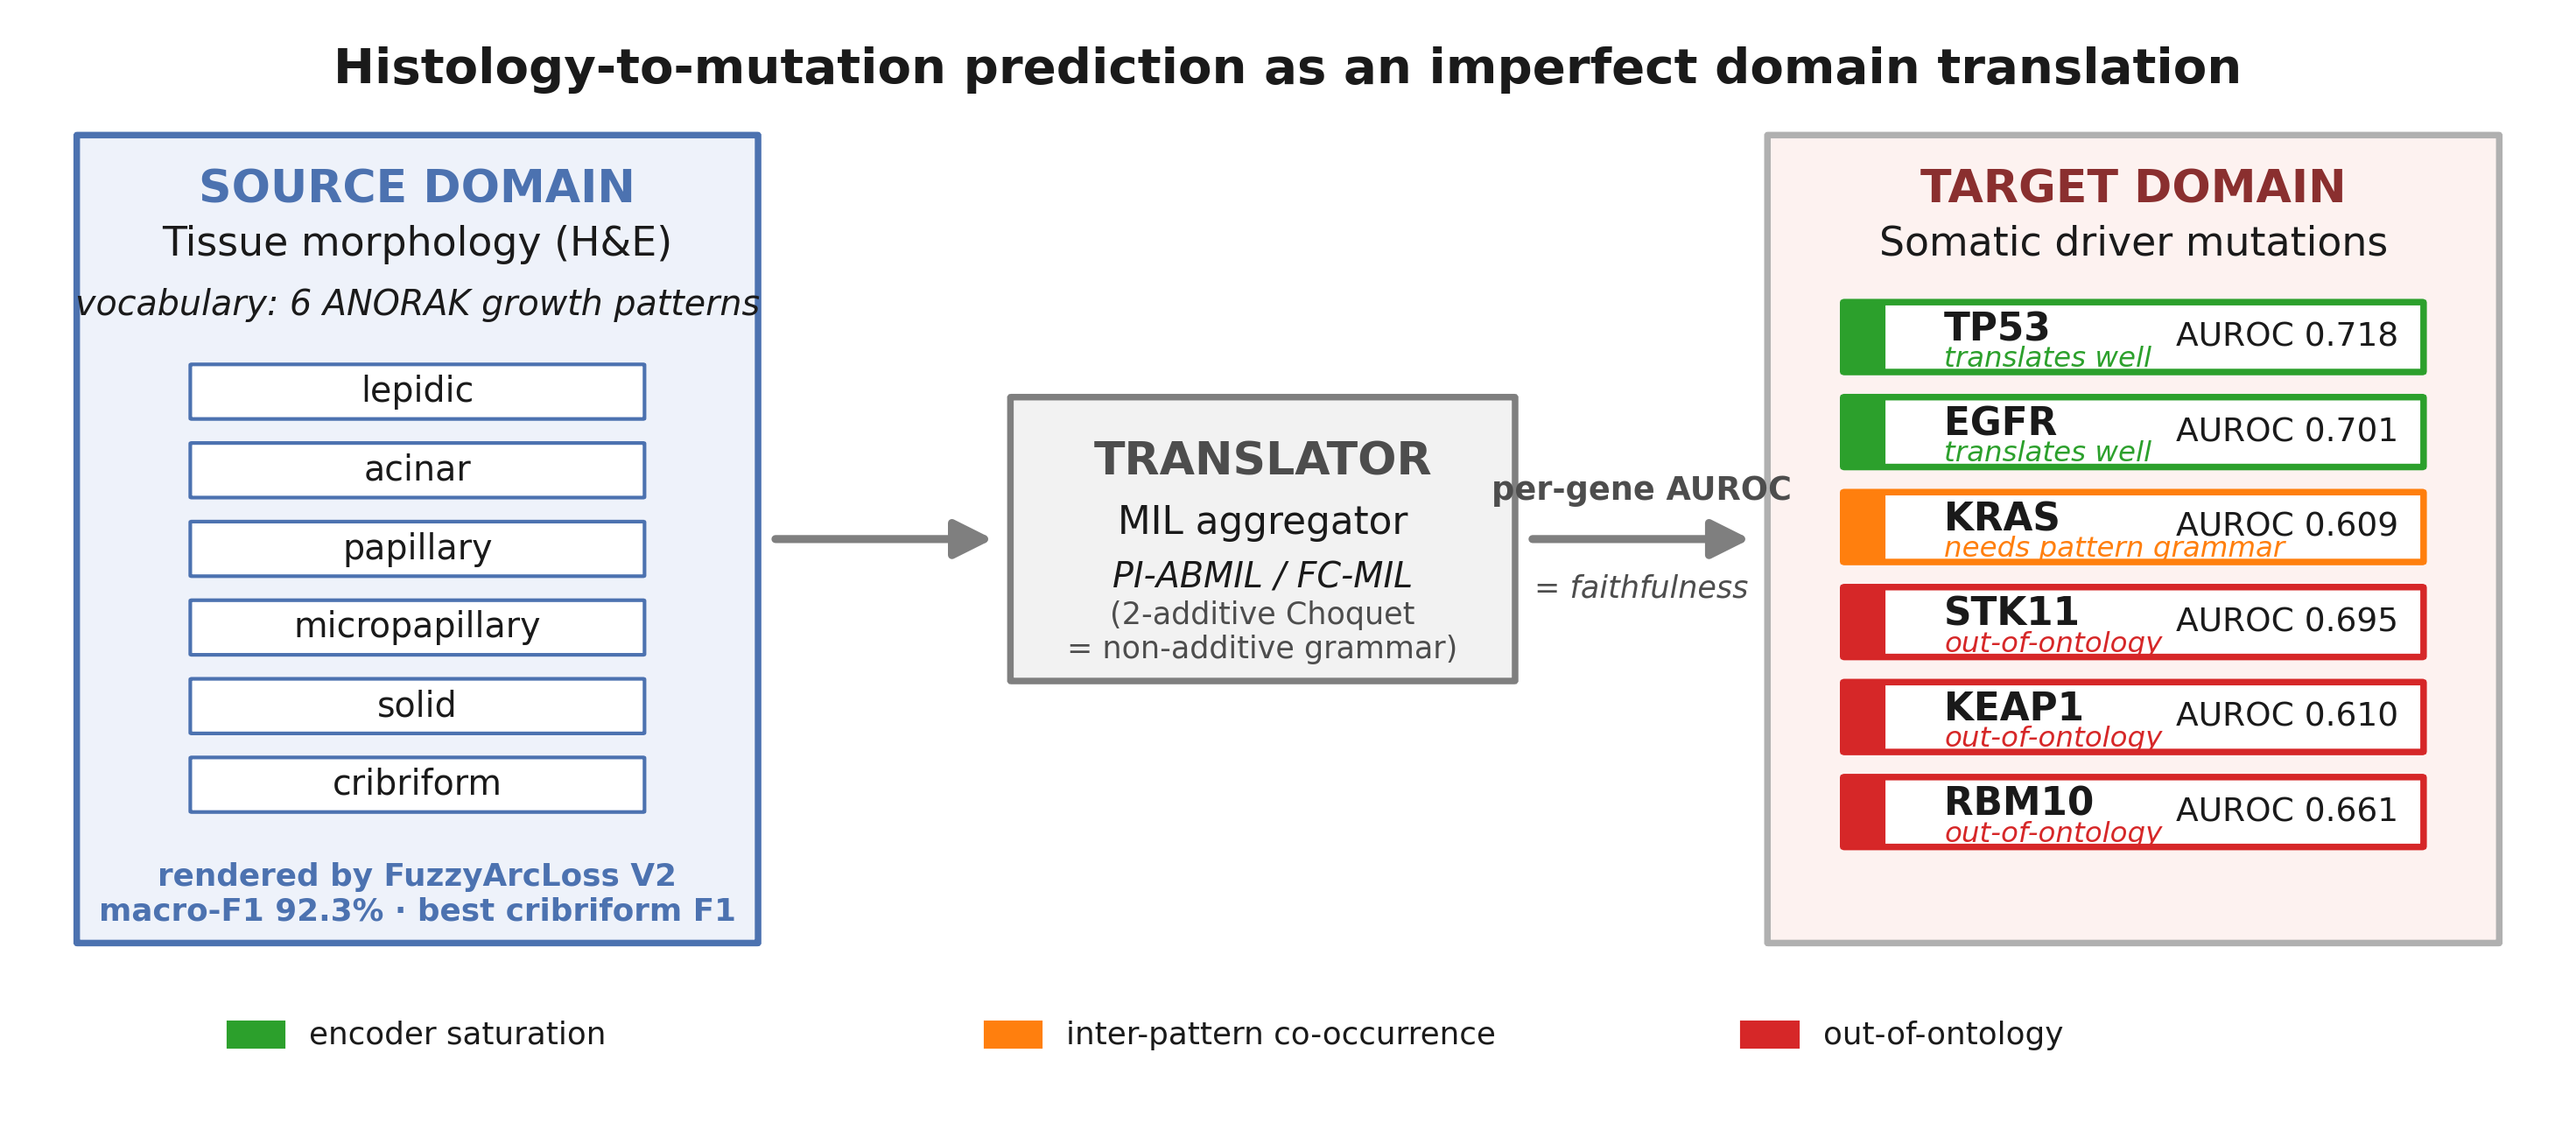
\includegraphics[width=\linewidth]{domain_translation_concept}
  \caption{\textbf{Cross-domain medical prediction as an imperfect
  translation, and the two channels over which it is decomposed.}
  \textbf{a}, A \emph{source} domain of tissue morphology, whose
  vocabulary is the six ANORAK growth patterns, is mapped by a
  multiple-instance translator onto a \emph{target} domain of somatic
  driver mutations; the per-target \auroc{} measures translational
  faithfulness averaged over the cohort. \textbf{b}, The two channels the
  aggregator receives. The morphology channel carries \ctranspath{} tile
  embeddings $\mathbf{h}_i$ into a gated-attention aggregator
  (\piabmil{}); the composition channel carries the $6$-d fuzzy pattern
  probabilities $\mathbf{p}_i$ into a $2$-additive Choquet integral
  (\fcmil{}). The two are disjoint until the classifier head, which is
  what makes \cref{eq:pid} well posed as a statement about two sources:
  neither channel can route information through the other, so an empty
  pattern-side atom cannot be an artefact of the architecture. Only the
  vocabulary and the encoder change when the framework moves to glioma MRI
  or to the electrocardiogram (\cref{fig:pipeline_glioma,fig:pipeline_ecg}).}
  \label{fig:framework}
\end{figure}
